\graphicspath{ {./Pictures/} }
%----------------------------------------------------------------------------------------
%	CHAPTER 2
%----------------------------------------------------------------------------------------
\chapterimage{band1.png}


\chapter{Trigonometry}

\subsection{Introduction}
Trigonometry is most simply associated with planar right-angle triangles (each of which is a two-dimensional triangle with one angle equal to 90 degrees). The applicability to non-right-angle triangles exists, but, since any non-right-angle triangle (on a flat plane) can be bisected to create two right-angle triangles, most problems can be reduced to calculations on right-angle triangles. Thus the majority of applications relate to right-angle triangles.
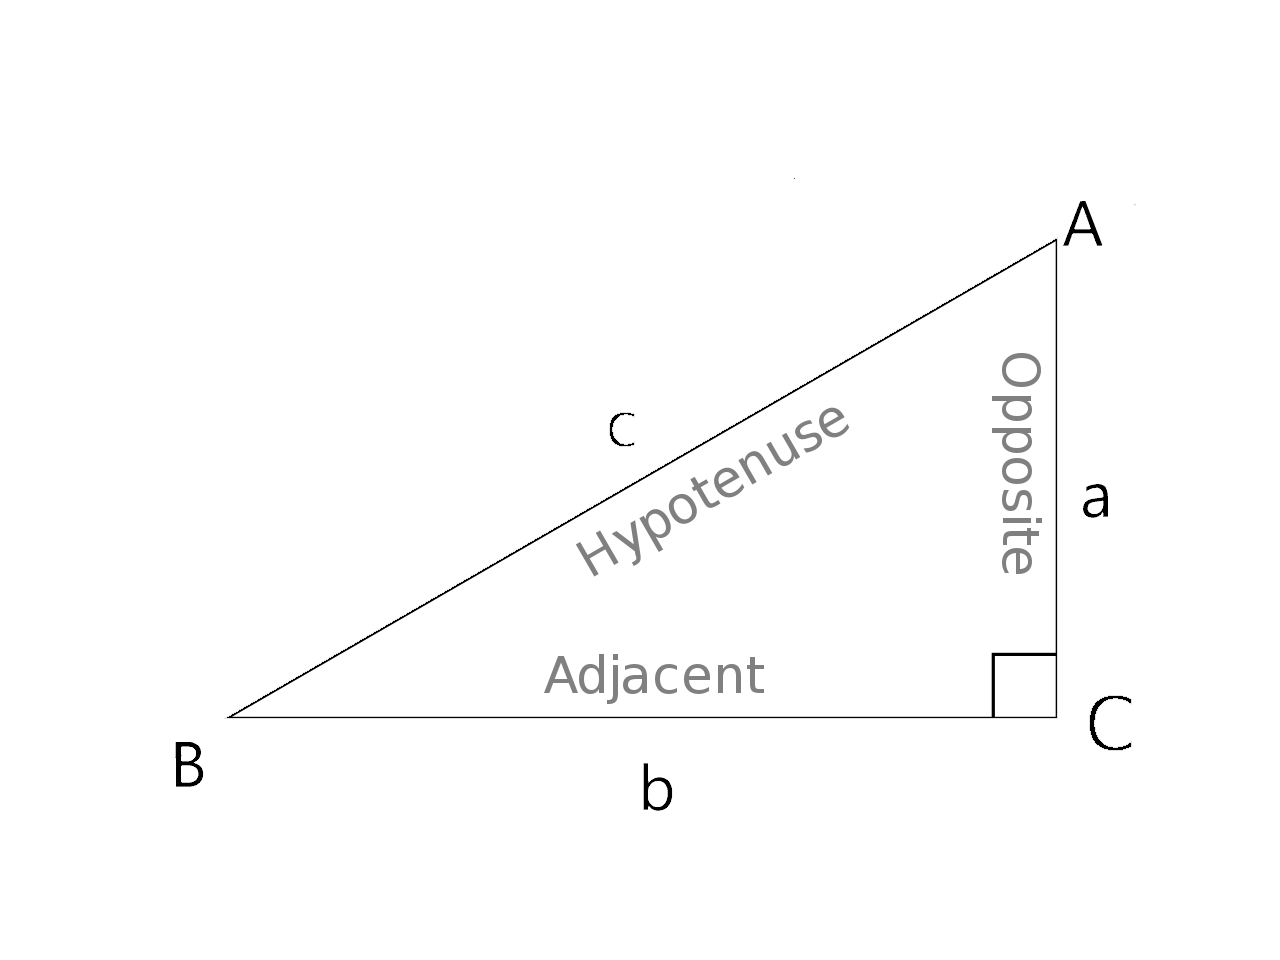
\includegraphics[width=50mm]{3}
One exception to this is spherical trigonometry, the study of triangles on spheres, surfaces of constant positive curvature, in elliptic geometry (a fundamental part of astronomy and navigation). Trigonometry on surfaces of negative curvature is part of hyperbolic geometry.
\newline
Define:
\newline
\begin{equation}
\sin\theta = \frac{Opposite}{Hypotenuse} = \frac{b}{c}
\end{equation}
\begin{equation}
\cos\theta = \frac{Adjacent}{Hypotenuse} = \frac{a}{c}
\end{equation}
\begin{equation}
\tan\theta = \frac{\sin\theta}{\cos\theta}= \frac{b/c}{a/c} = \frac{Opposite}{Adjacent} = \frac{b}{a}
\end{equation}
\newpage
Example: 1
\begin{equation}
a^2+b^2=c^2
\end{equation}
\begin{displaymath}
=>\frac{a^2}{c^2}+\frac{b^2}{c^2} = 1
\end{displaymath}
\begin{displaymath}
=> \bigg(\frac{a}{c}\bigg)^2 + \bigg(\frac{b}{c}\bigg)^2 = 1
\end{displaymath}
\begin{displaymath}
=> (\cos\theta)^2+(\sin\theta)^2 = 1
\end{displaymath}
\begin{equation}
\cos^2\theta+\sin^2\theta = 1
\end{equation}
\newline
\begin{equation}
Cotangent->\cot\theta = \frac{1}{\tan\theta} = \frac{a}{b} = \frac{\cos\theta}{\sin\theta}
\end{equation}
\begin{equation}
Secant->\sec\theta = \frac{1}{\cos\theta} = \frac{c}{a}
\end{equation}
\begin{equation}
Cosecant->\cosh\theta = \frac{1}{\sin\theta}=\frac{c}{b}
\end{equation}
\newline
Example: 2
\begin{equation}
a^2+b^2=c^2
\end{equation}
\begin{displaymath}
=>1+\frac{b^2}{c^2}=\bigg(\frac{c}{a}\bigg)^2
\end{displaymath}
\begin{displaymath}
=> 1+\bigg(\frac{b}{a}\bigg)^2=\bigg(\frac{c}{a}\bigg)^2
\end{displaymath}
\begin{displaymath}
=> 1+\tan^2\theta = \sec^2\theta
\end{displaymath}
\newline
Example: 3
\begin{equation}
a^2+b^2=c^2
\end{equation}
\begin{displaymath}
=>\frac{a^2}{b^2}+1 = \frac{c^2}{b^2}
\end{displaymath}
\begin{displaymath}
=> \bigg(\frac{a}{b}\bigg)^2+1= \bigg(\frac{c}{b}\bigg)^2
\end{displaymath}
\begin{displaymath}
=> \cot^2\theta+1=\cosh^2\theta
\end{displaymath}

\subsection{Compound angle in trigonometry function}
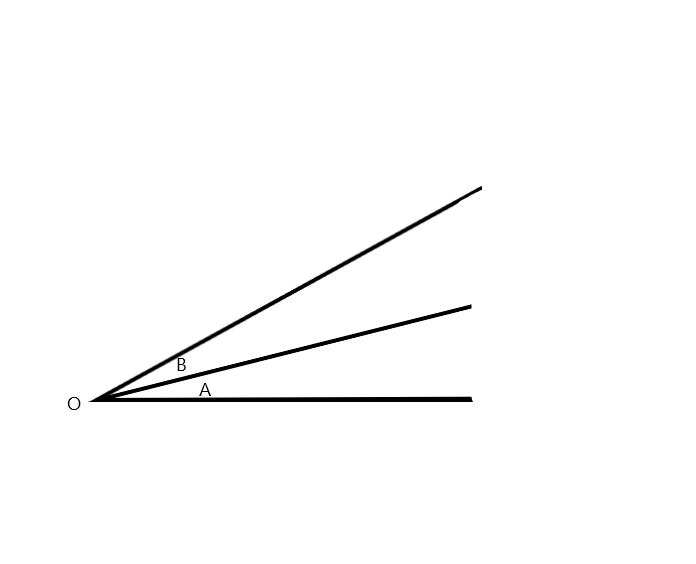
\includegraphics[width=60mm]{5}
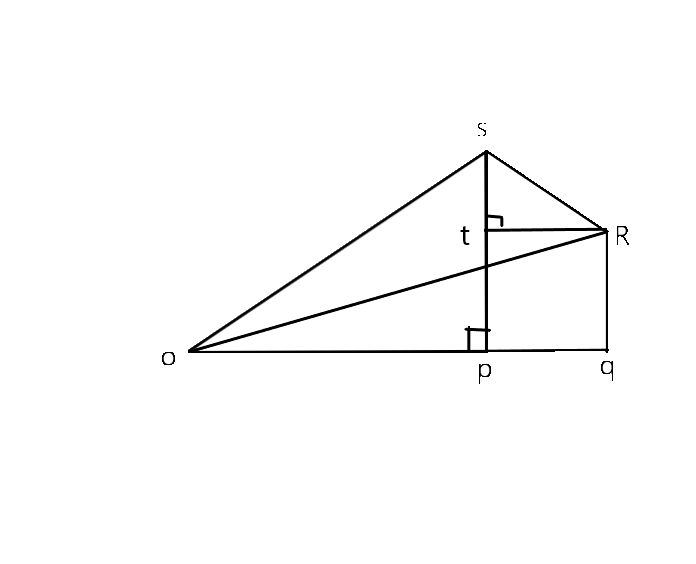
\includegraphics[width=60mm]{4}
\newline
Example
\begin{equation}
\sin(A+B)=\frac{sp}{os}
\end{equation}
\begin{displaymath}
=>\frac{st+tp}{os}
\end{displaymath}
\begin{displaymath}
=>\frac{st}{os}+\frac{tp}{os}
\end{displaymath}
\begin{displaymath}
=>\frac{st}{sr}\frac{sr}{os}+\frac{tp}{os}
\end{displaymath}
\begin{displaymath}
=>\frac{st}{sr}\frac{sr}{os}+\frac{ra}{or}\frac{or}{os}
\end{displaymath}
\begin{displaymath}
=> \cos A\sin B+\sin A\cos B
\end{displaymath}
\begin{equation}
\sin(A+B) = \sin A\cos B+\cos A\sin B
\end{equation}

\subsection{Differentiation of trigonometric functions}
\begin{equation}
\sin(A+B) = \sin A\cos B+\cos A\sin B
\end{equation}
\begin{equation}
\cos(A+B) = \cos A\cos B - \sin A\sin B
\end{equation}
\begin{equation}
\frac{df(x)}{dx} = \frac{f(x+h)-x}{h}
\end{equation}
\newline
Example: 1
\begin{displaymath}
\frac{d\sin(x)}{dx} = \frac{\sin x \cos h+\cos x\sin h-\sin x}{h}
\end{displaymath}
\begin{displaymath}
=> \frac{\sin x + h\cos x - \sin x}{h}
\end{displaymath}
\begin{displaymath}
=>\frac{h\cos x}{h}
\end{displaymath}
\begin{equation}
\frac{d\sin(x)}{dx} = \cos x
\end{equation}
\newline
Example: 2
\begin{displaymath}
\frac{d\cos(x)}{dx} = \frac{\cos(c+h)-\cos (x)}{h}
\end{displaymath}
\begin{displaymath}
=> \frac{\cos x \cos h-\sin x \sin h - \cos x}{h}
\end{displaymath}
\begin{displaymath}
=> \frac{cos x- h \cos x - \cos x}{h}
\end{displaymath}
\begin{displaymath}
=> \frac{-h\sin x}{h}
\end{displaymath}
\begin{equation}
\frac{d\cos (X)}{dx} = -\sin x
\end{equation}
\newline
Example: 3
\begin{displaymath}
\frac{d\tan x}{dx}
\end{displaymath}
\begin{displaymath}
=>\frac{d}{dx}\bigg(\frac{\sin x}{cos x}\bigg)
\end{displaymath}
\begin{displaymath}
=>\frac{d}{dx}(\sin x)\frac{1}{\cos x}+\sin x \frac{d}{dx}\bigg(\frac{1}{\cos x}\bigg)
\end{displaymath}
\begin{displaymath}
=>\cos x \frac{1}{\cos x}+\sin x\frac{d}{dx}(\cos x)^{-1}
\end{displaymath}
\begin{displaymath}
=> 1+\sin x\bigg[(-1)(\cos x)^{-2}\frac{d\cos x}{dx}\bigg]
\end{displaymath}
\begin{displaymath}
=> 1+\sin x\frac{-1}{\cos x^2}(-\sin x)
\end{displaymath}
\begin{equation}
\frac{d \tan x}{dx} = 1 + \tan^2 x
\end{equation}

